
\section{Appendix}

\todo{Appendices: Supplementary materials could be included.  Each appendix must be labeled (for example, Apeendix A, Appendix B) and with heading.  All Appendices must be referred to in the text.  }
\subsection{ECOG performance status}
\todo{Oken M, Creech R, Tormey D, \textit{et al.} Toxicity and response criteria of the Eastern Cooperative Oncology Group. Am J Clin Oncol. 1982;5:649-655.}


\begin{tabular}{|l p{8cm}|}
\hline
GRADE&	ECOG PERFORMANCE STATUS\\
\hline\hline
0	&Fully active, able to carry on all pre-disease performance without restriction\\
1	&Restricted in physically strenuous activity but ambulatory and able to carry out work of a light or sedentary nature, e.g., light house work, office work\\
2	&Ambulatory and capable of all selfcare but unable to carry out any work activities; up and about more than 50\% of waking hours\\
3	&Capable of only limited selfcare; confined to bed or chair more than 50\% of waking hours\\
4	&Completely disabled; cannot carry on any selfcare; totally confined to bed or chair\\
5	&Dead\\
\hline
\end{tabular}
\label{tab:ecog}


\subsection{Projectplan}
\begin{sidewaysfigure}[h]
	\centering
	\includegraphics[page=2,width=\textwidth]{appendix/Projectplan.pdf}
	\caption{Detailed description and properties of single task listed in the project plan (Page 1/2)}
	\label{fig:projectplan:details:1}
\end{sidewaysfigure}

\begin{sidewaysfigure}[h]
	\centering
	\includegraphics[page=3,width=\textwidth]{appendix/Projectplan.pdf}
	\caption{Detailed description and properties of single task listed in the project plan (Page 2/2)}
	\label{fig:projectplan:details:2}
\end{sidewaysfigure}


\section{Software related appendix}
\subsection{Installation Guide}
\label{app:installation}
\todo{Write Installation Guide}

\subsection{Use Cases}
\label{app:use_cases}
\todo{export usecases from trello}

\subsection{Structure of application}
\label{app:structure}
\todo{Component diagram}